% !TeX root = ../main.tex
% Add the above to each chapter to make compiling the PDF easier in some editors.

\section{Foveated Rendering}
\subsection{Theory}
This technique lends its name from the \textit{fovea centralis}, a spot in the center of the human retina, responsible for sharp central vision of the eye. The regions around it gradually lose visual sharpness as they contain fewer and fewer cone cells. 
Foveated rendering in its various forms builds on this limitation of the human photoreceptive system. For example described in the Oculus Go optimization guide \cite{Palandri.2018}, the image produced by a VR renderer is warped by the VR compositor to more closely match the spherical shape of the lenses and the distorted field of view they create. This warping means that toward the edge of the frame, more pixels are compressed into a given angle of vision than in the center, effectively leading to much higher pixel density for peripheral regions. \\
Conversely, the peripheral vision of the human eye is commonly significantly less sharp than aforementioned foveal vision. So it seems logical that the outer rim of the rendered image could be rendered at much lower pixel density without sacrificing a \textit{humanly noticeable} amount of detail. 
Exactly that is the concept of foveated rendering, to decrease resolution of the edge regions of the image while rendering the central area at full resolution. 
There is one big constraint, however. The foveal vision of the user and the artificial foveal center of the image need to match up, otherwise a user may easily notice the lowered pixel density. To accurately match these two focus points, the user's eye movements need to be tracked and the supposed focus center of the image adjusted accordingly. 

\subsubsection{Fixed versus "True" Foveated Rendering}
Eye tracking can be foregone in theory, assuming the headset's field of view is low enough to physically discourage a wide range of eye movement and instead rely on head rotation. Additionally, the opening angle of the foveated region should be wider so eye movement on a small scale is still without consequence to the perceived image quality. And the resolution of peripheral areas may not be reduced as much as with "true" foveated rendering so even when the user briefly looks at such an area, the perceived loss is not as distracting. This compromise form of the technique is commonly called Fixed Foveated Rendering, for example available on Oculus Go (\autoref{fig:Oculus_FFR}). \\
Given eye tracking of some adequate sort is available, "true" FR can be performed, where in each frame the current focus position of each eye is queried and the virtual view matrix updated accordingly. This makes the rendering setup more complex, of course, as the high pixel density area can shift to any location within the image, but it possibly allows for a tighter foveal angle and lower peripheral resolution as it is much less likely - if not entirely impossible due to limits or occasional mistakes by the tracker - for the user to focus on any such low density frame data. See ZeroLight Limited's Nvidia VRS based approach in \autoref{fig:ZeroLight_DFR}. \\

\begin{figure}[!ht]
     \subfloat[Oculus Go Fixed Foveated Rendering map (colored tiles decrease in resolution outward)\cite{Palandri.2018}\label{fig:Oculus_FFR}]{%
       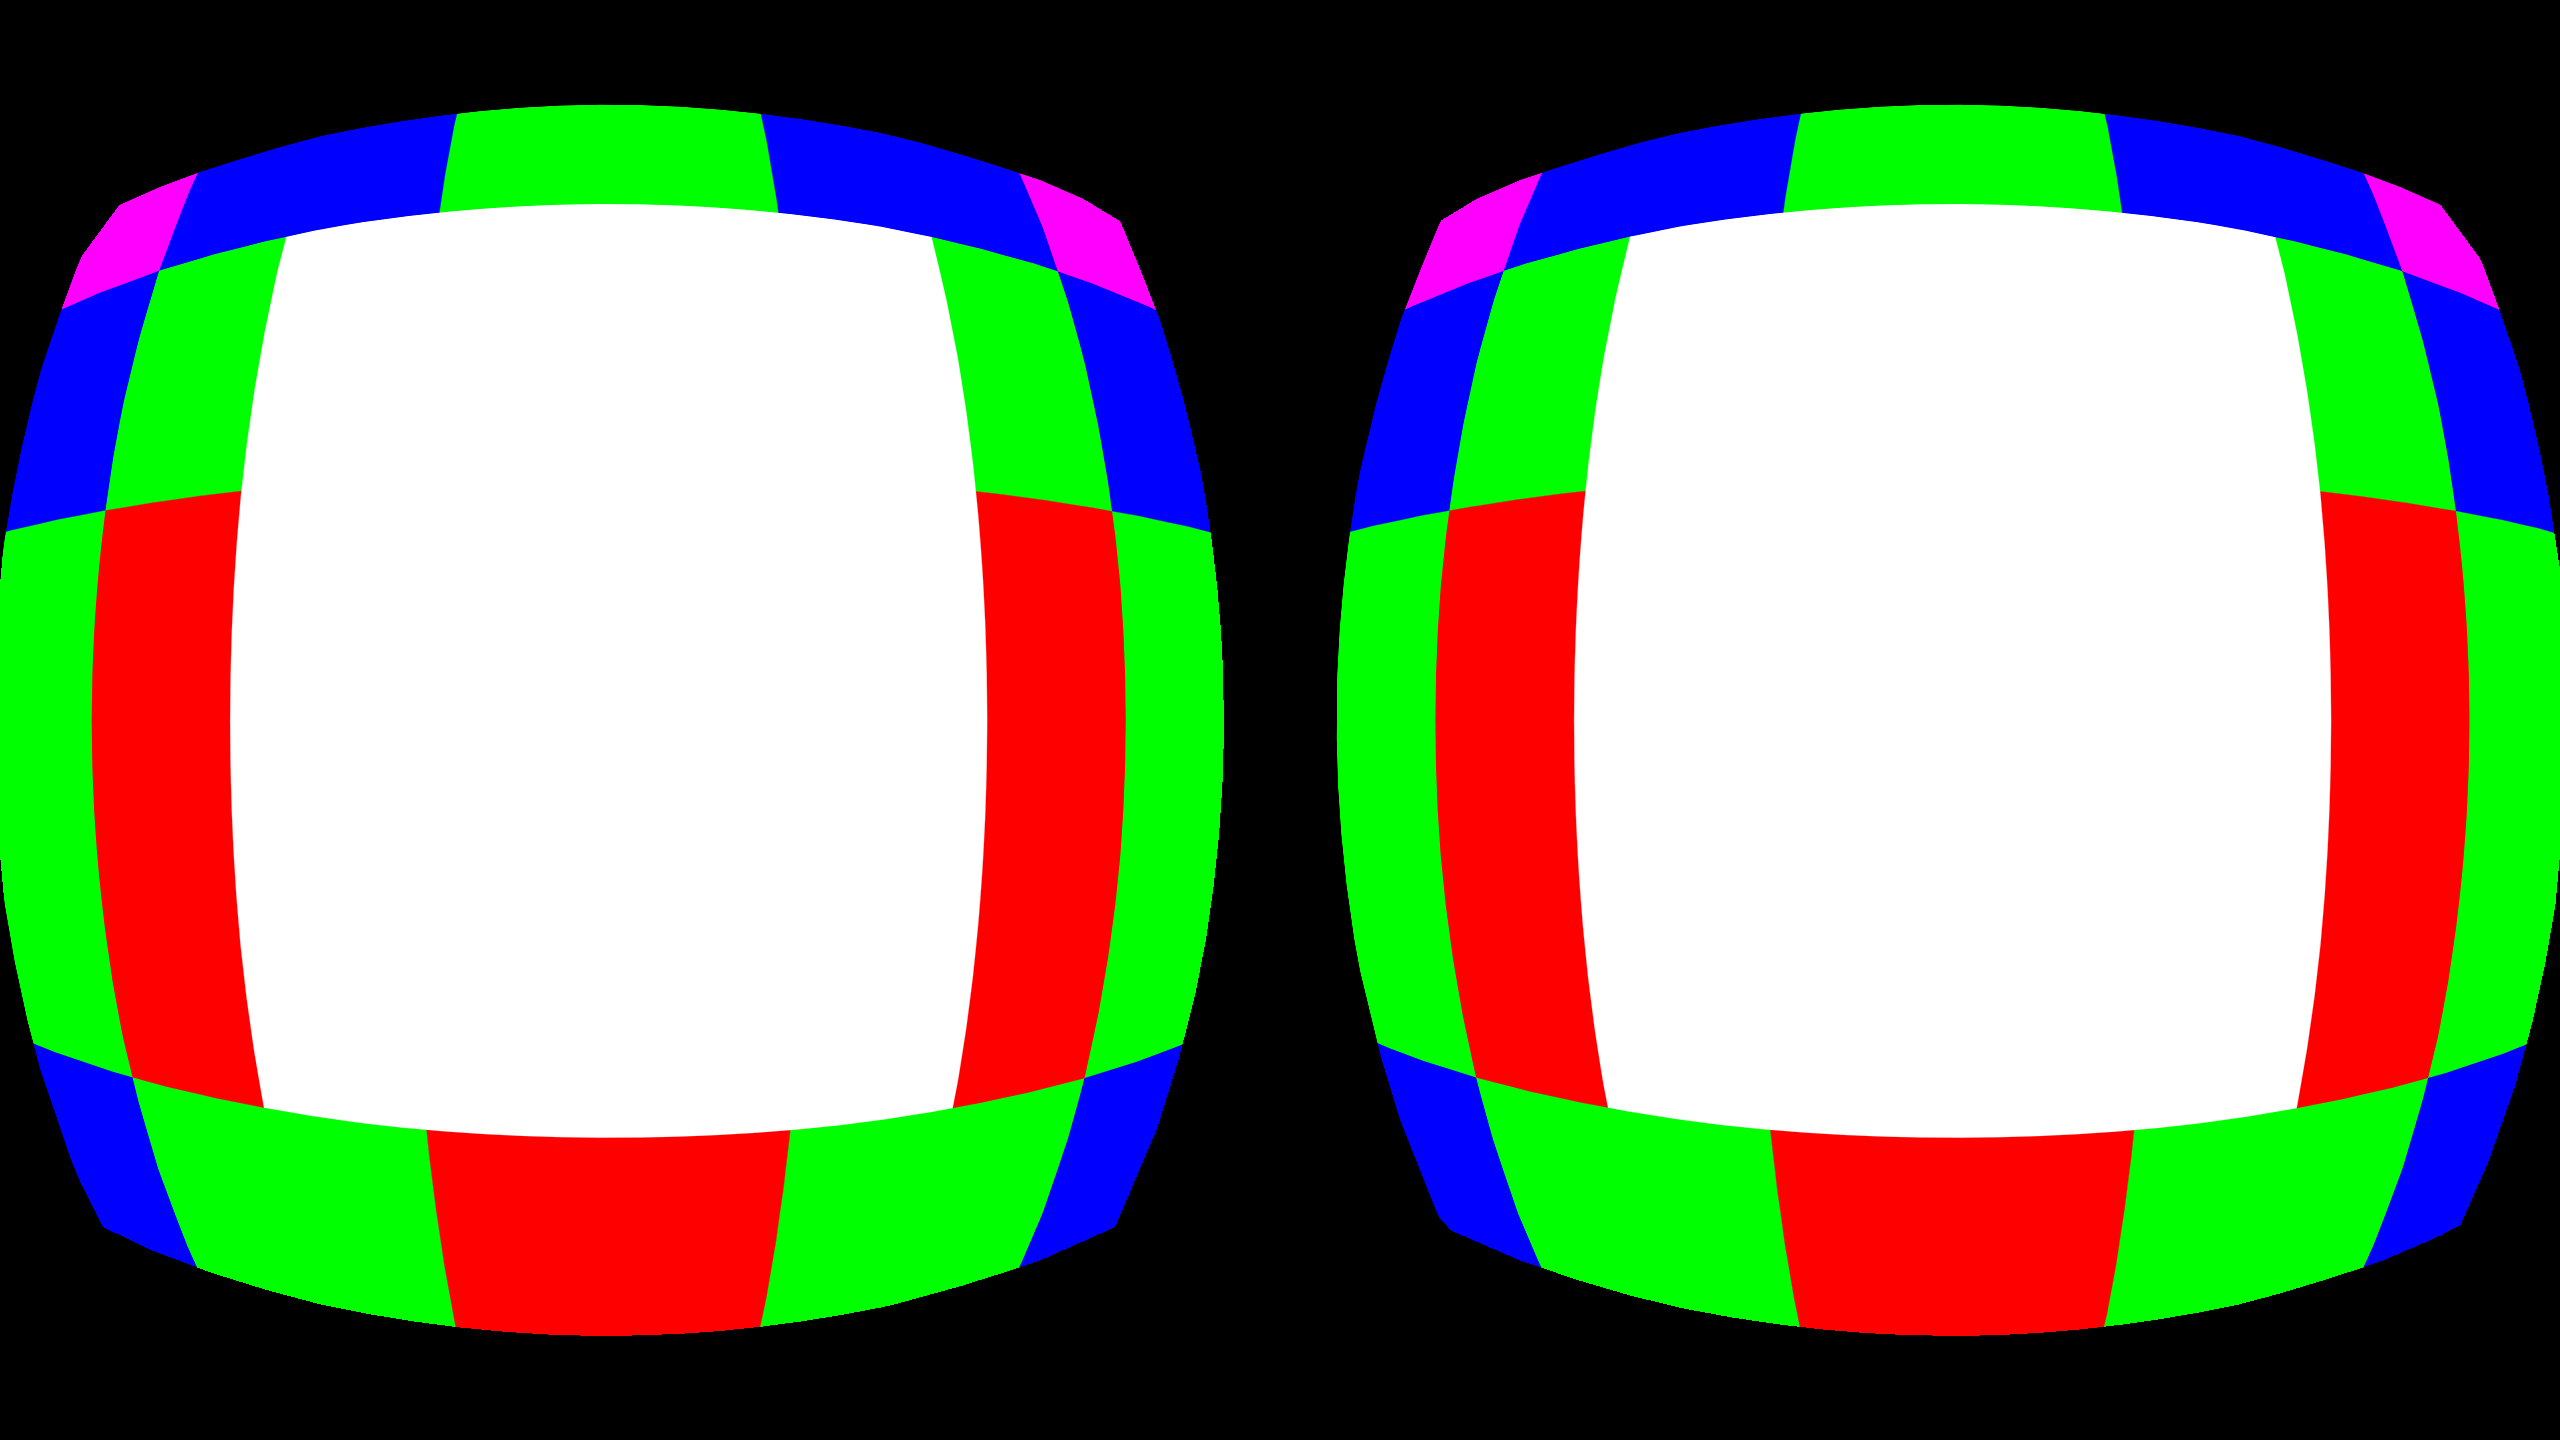
\includegraphics[width=0.9\textwidth]{pictures/Oculus_Go_FFR}
     }
     \hfill
     \subfloat[Dynamic Foveated Rendering using Nvidia Variable Rate Shading on HTC Vive Pro Eye\cite{ZeroLightLimited.2019}\label{fig:ZeroLight_DFR}]{%
       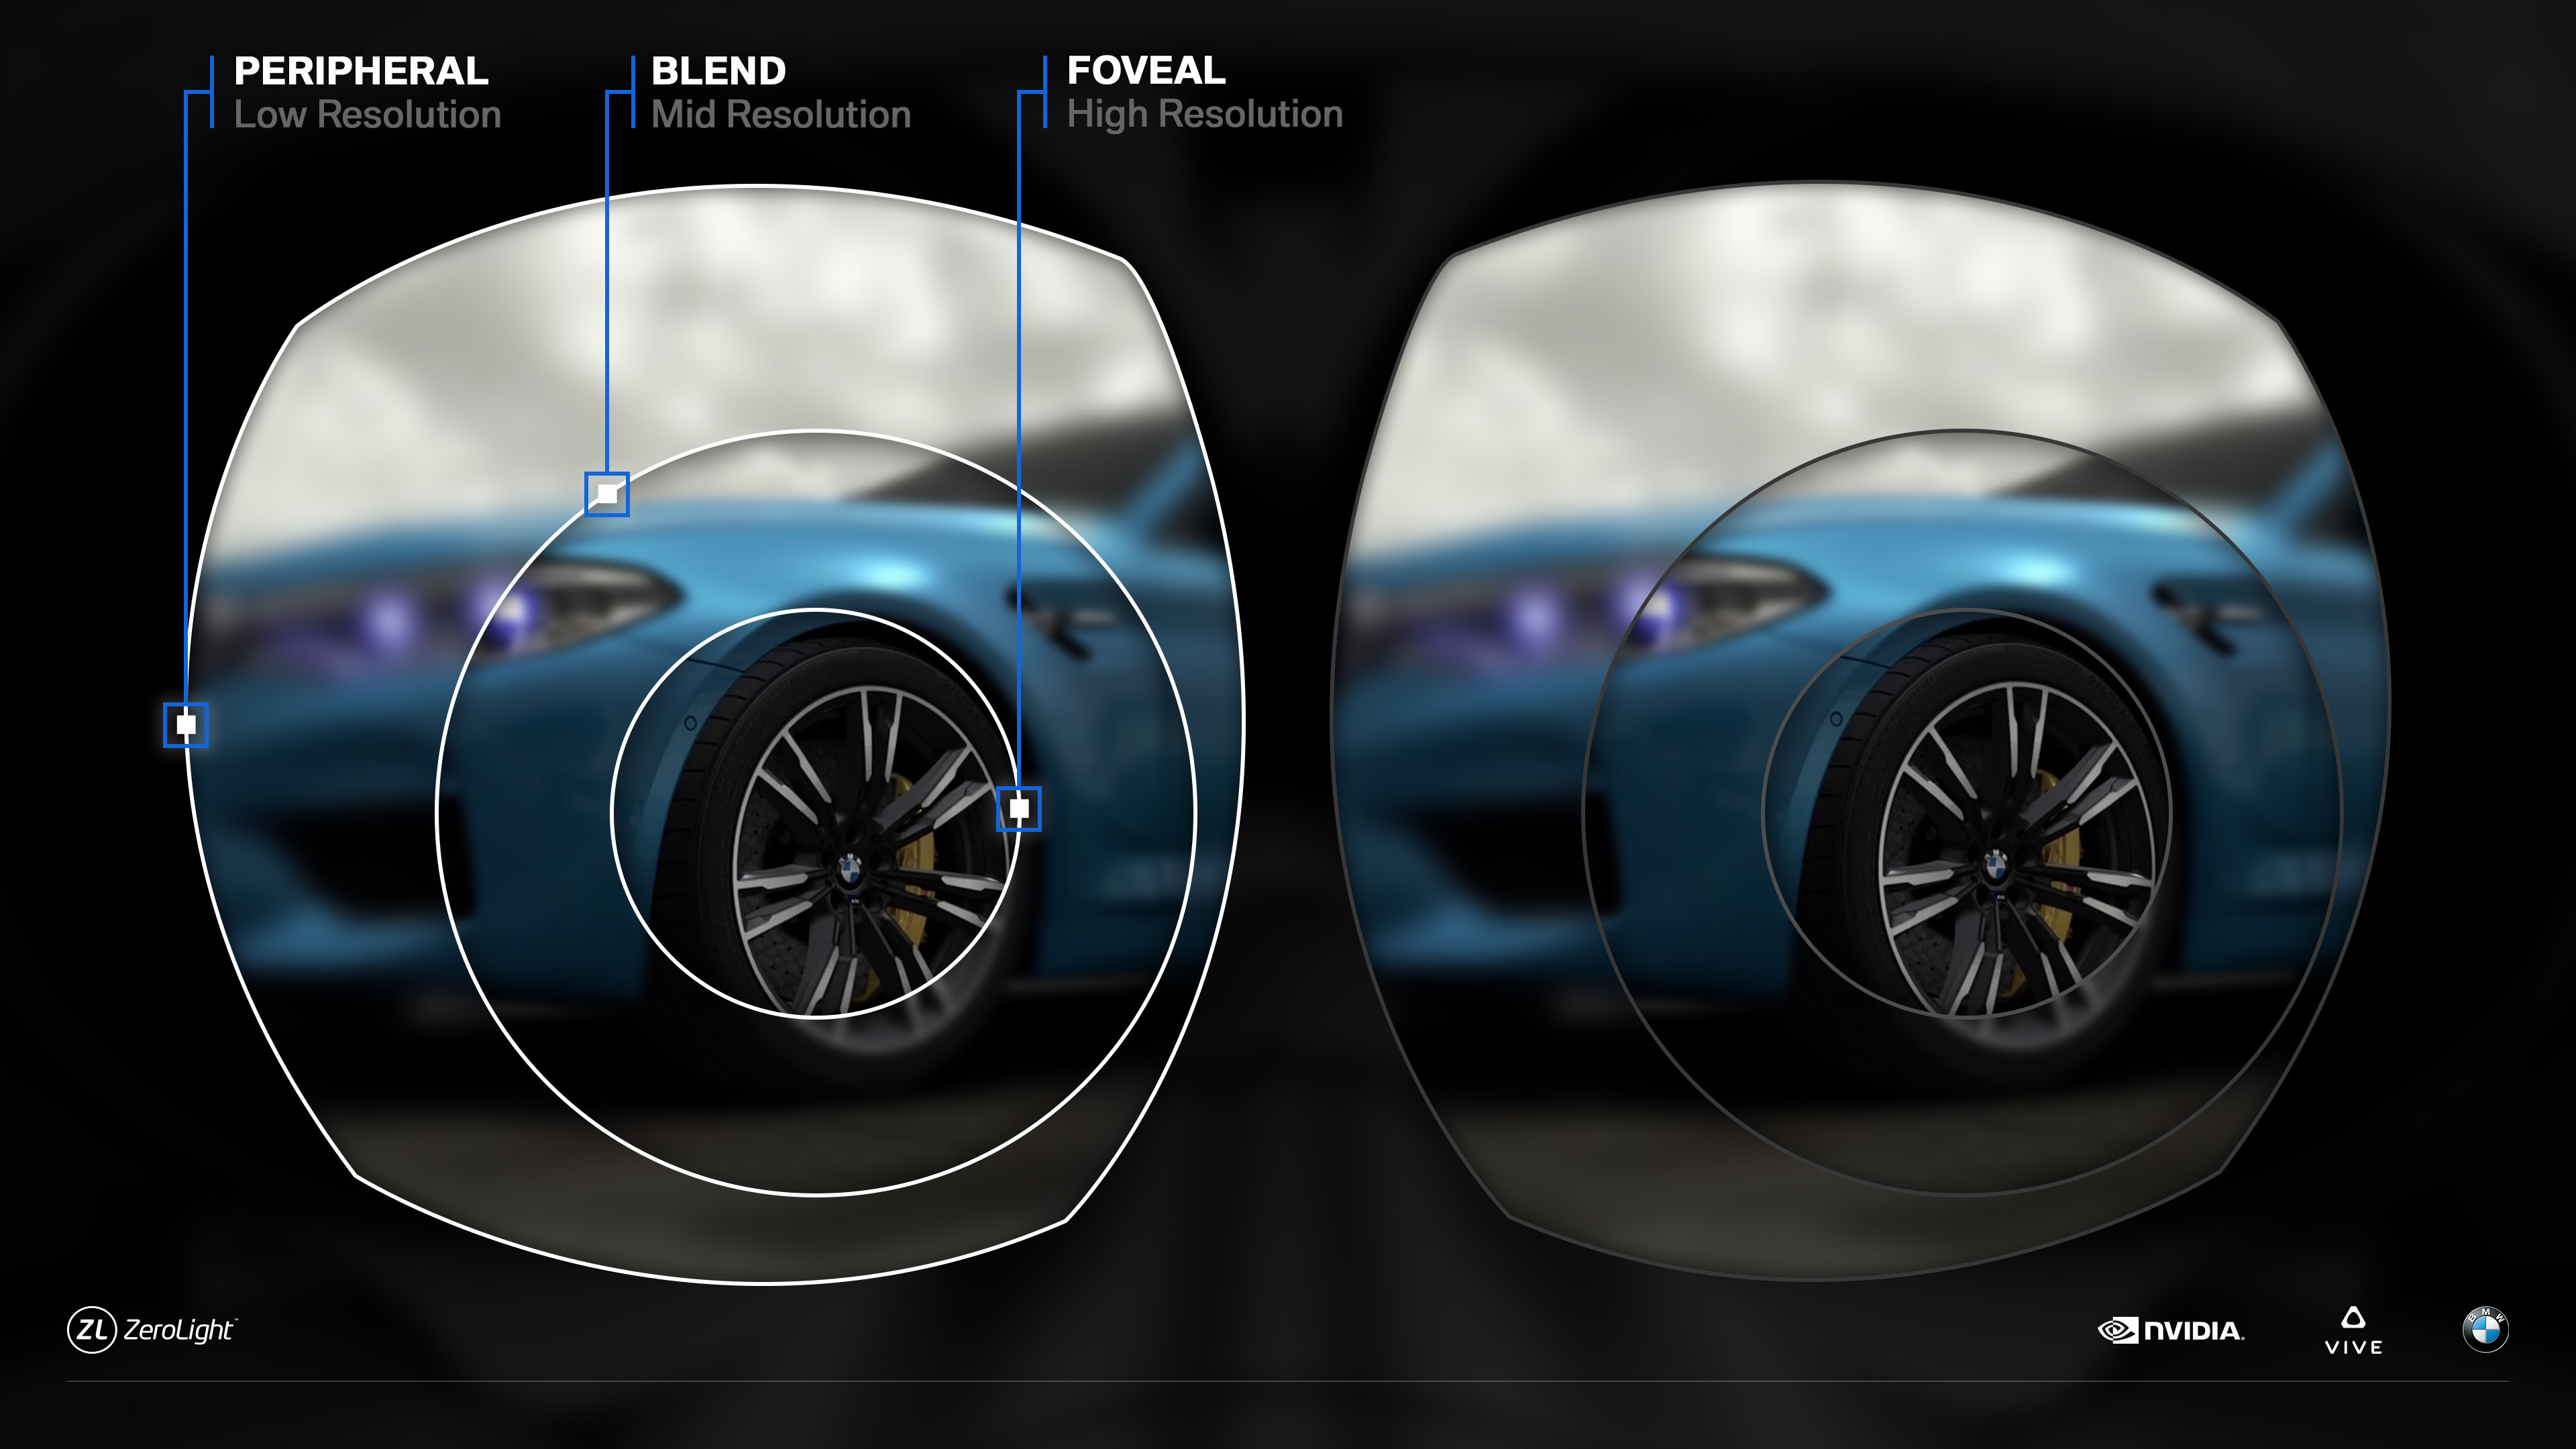
\includegraphics[width=0.9\textwidth]{pictures/ZeroLight_DFR}
     }
     \caption{Foveated rendering examples}
     \label{fig:FovRendering}
\end{figure}

\subsection{Radial Density Mask}
A somewhat related technique is called radial density masking as also shown by Valve's Alex Vlachos in his \cite{Vlachos.2016c}. The goal is the same as with FR, but the approach is different. Instead of reducing the theoretical rendering resolution of the peripheral ring, a mask is overlaid that has the render pipeline skip a certain pattern of pixels in that ring. This could, for example, be done by marking a checkerboard pattern of pixels in the stencil buffer so the pixel shaders fails the stencil test on them - coming back to \autoref{stencilmask} - to get a pixel perfect mask, or by overlaying a masking mesh right at the near plane of the render volume so the respective fragments are discarded during early Z tests. The latter way would allow to approximately match a relative reduction target, but may not be pixel perfect depending on internal frame resolution. 
The resulting checkerboard area can then be interpolated and filtered to reconstruct the missing information. 
Vlachos cites gains of up to 15\% for the Valve Aperture Robot Repair demo scene, but warns that reconstruction cost needs to be kept lower than mask savings of course. \\

\begin{figure}[!htb]
  \centering
  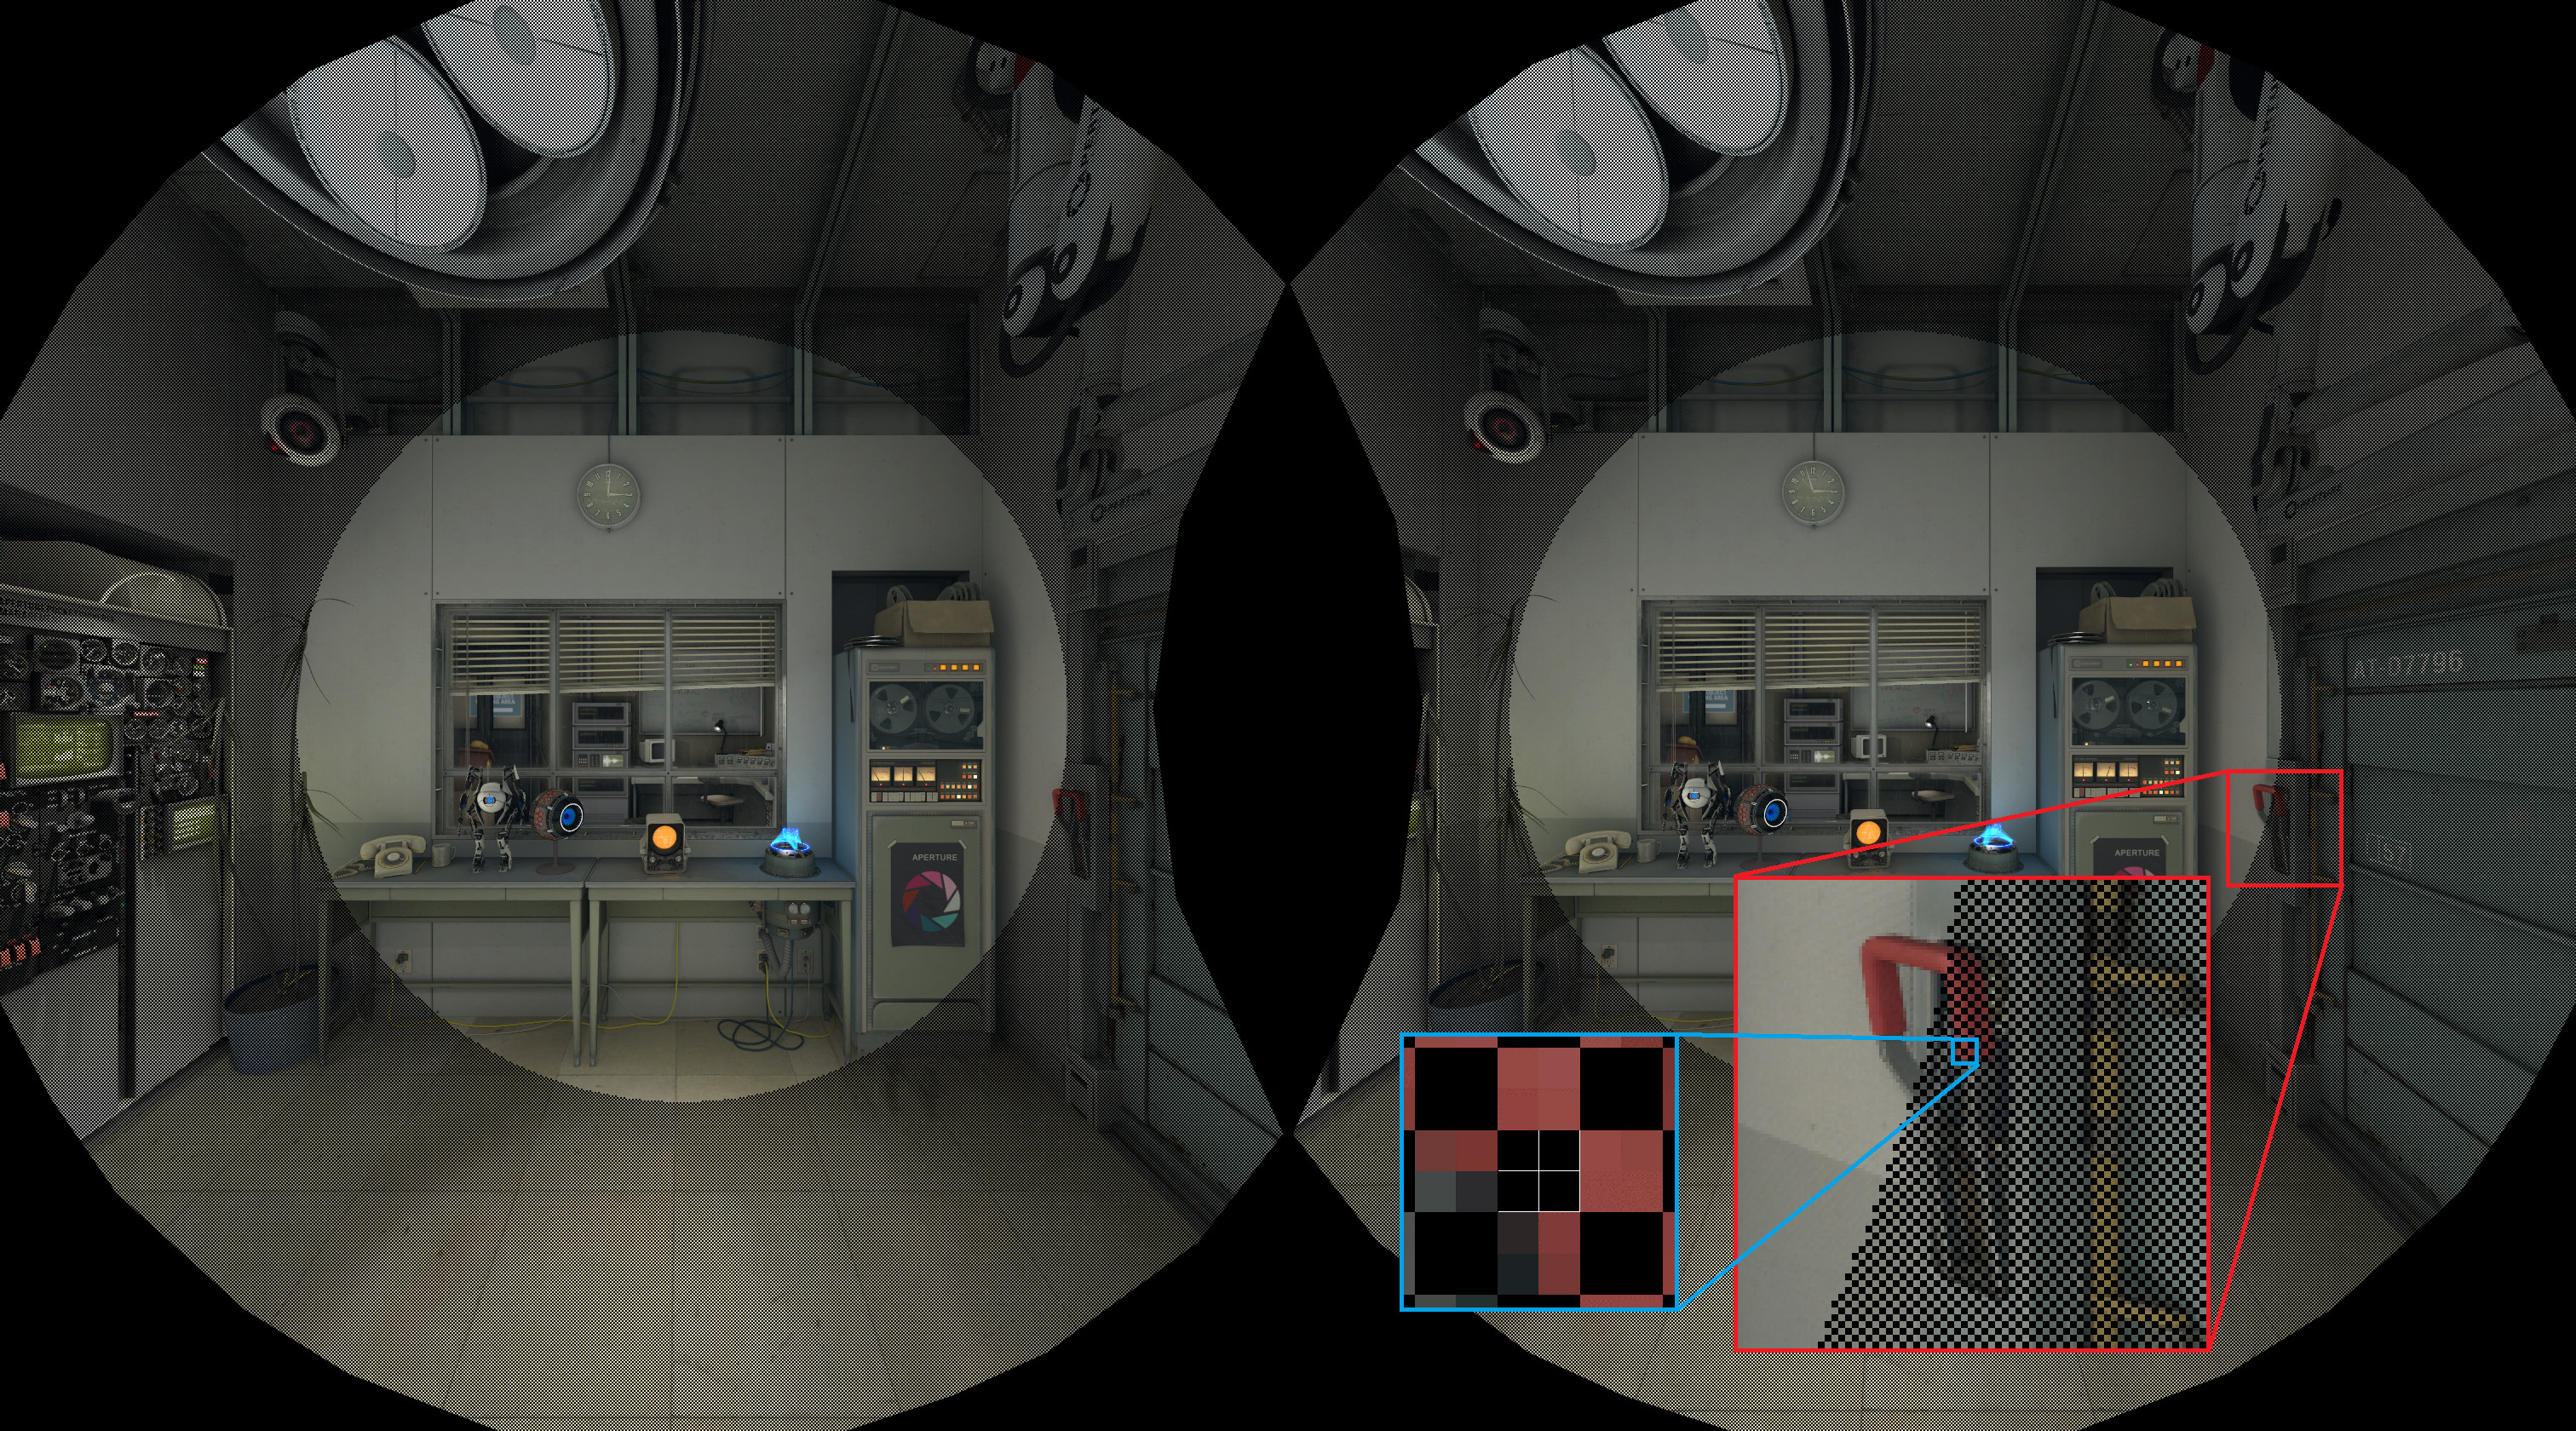
\includegraphics[width=0.9\textwidth]{pictures/vlachos_RDM}
  \caption{Radial Density Masking (2x2 px checkerboard)\cite{Vlachos.2016c}} \label{fig:vlachos_RDM}
\end{figure} 

\subsubsection{Adaptive resolution}
The described methods of FFR, FR and RDM can of course be combined further with another, by now almost universal, optimization compromise: dynamic resolution. While monitoring GPU load or frametimes and framepacing, the resolution of not just the central fovea but obviously the peripheral regions could be reduced or increased within given bounds as these metrics allow. This can stabilize performance at the cost of some visual quality in the outer regions, or at the other end of the spectrum alleviate some of the quality reduction if the available power overhead allows. 

\subsubsection{Relevancy of GPU architecture}
The previous sections describe various methods, but the choice of which is ideal for a given engine depends a lot on the target hardware. Foveated rendering relies on splitting the frame into several rectangular sub-frames and rendering them at differing internal resolution. Thus, FR is only suited for GPU architectures supporting or better yet being built as so-called tile based renderers. Tile based GPUs such as Qualcomm's Adreno line and most other low power mobile SoCs compute the frame in parallel in a number of set tiles as opposed to traditional GPUs which execute render commands in sequence and can only work on a frame as one entire unit, albeit with possibly many more compute units at once. These tile based architectures naturally make it very simple to render tiles outside the fovea at lower resolution, with the fovea circle being better approximated the higher the tile count is. \\
More traditional architectures like those found in Nvidia and AMD desktop graphics chipsets are rarely built as tile renderers and may only support this tiling in software. On those, rendering frame regions at different resolutions requires multiple render passes in sequence with a subsequent composition pass that writes the multiple layers into a single frame. This sequential process incurs additional overhead and may not yield ideal core utilization if the low resolution pass does not provide enough work for a large number of shader cores. The radial density mask approach may be more suitable for such traditional GPUs as it manages to render multiple resolutions within a single render pass by leveraging fragment discard features. This masking will necessitate an interpolation pass to blend away the masked pixels, while foveated rendering can technically skip further interpolation. Filtering the low resolution perifoveal pixels is recommended though to reduce aliasing. \\

\textcolor{red}{[TODO: illustration Tile vs Whole?]}